\documentclass{article}[18pt]
\usepackage{../../../../format}
\lhead{Software Methodologies - Computer Graphics}
\usepackage{minted}


\begin{document}
\begin{center}
\underline{\huge Scene Construction and Projection}
\end{center}
\section{World and Local Coordinate Systems}
\textbf{Local Coordinates} - Each object is constructed on a dedicated coordinate system\\
\\
\textbf{World coordinates} - Apply a single coordinate system to all objects globally.\\
\\
The purpose of this is to reduce complication for 3D scene construction
\section{View Transform}
Shift the origin of the world coordinate system to the view origin. The view origin is where our eye (or virtual camera) is located with respect to the world origin\\
\\
The purpose of this is to allow a user (application) to specify how 2D rendered images of a 3D scene will be generated
\section{Projection Transform}
\textbf{Visible Region} - Define which part of a 3D scene will be currently visible\\
\\
\textbf{Object appearance} - Modify or preserve object shape properties
\begin{center}
	\includegraphics[scale=0.7]{"Projection Transform"}
\end{center}
\section{Define a view frustum}
Projection transform is done based on a view frustum and it is defined by six planes (near, far, top, bottom, right and left)

\begin{center}
	\includegraphics[scale=0.3]{"View Frustum"}
\end{center}
\section{Types of View Frustum}
\begin{itemize}
	\item The shape and extent of the frustum determines the type of view projection from the 3D scene space to the 2D screen
	\item If the far and near planes have the same dimensions, then the frustum will determine an orthographic projection. Otherwise, it will be a perspective projection
\end{itemize}

\begin{center}
	\includegraphics[scale=0.5]{"Frustum Shape"}
\end{center}
\section{Viewport Transform}
Map projected view to the available space in the computer screen, i.e. viewport, typically referring to the canvas
\begin{center}
	\includegraphics[scale=0.7]{"Viewport Transform"}
\end{center}
\textbf{NDC} - Normalized Device Coordinates. Its x and y coordinates represent the location of your vertices on a normalised 2D screen space
\section{Model-View-Projection Transformation}
\begin{center}
	\includegraphics[scale=0.7]{"Model-View-Projection Transformation"}
\end{center}
\section{WEBGL - setLookAt()}
This takes the parameters: Eye Position, Look-at Position, Camera Orientation
\begin{itemize}
	\item Eye Position - $(x_{eye},y_{eye},z_{eye})$
	\item Look-at Position - $(x_{at},y_{at},z_{at})$
	\item Camera Position - $(dir_{x},dir_{y},dir_{z})$
\end{itemize}
Usage:
\begin{minted}{javascript}
// Set the matrix to be used to set the camera view
var viewMatrix = new Matrix4();
viewMatrix.setLookAt(0.20,0.25,0.25,0,0,0,0,1,0)

// Set the view matrix
gl.uniformMatrix4fv(u_ViewMatrix, false, viewMatrix.elements);

// Draw the rectangle
gl.drawArrays(gl.TRIANGLES, 0, n);
\end{minted}
\section{WebGL - setPerspactive}
\begin{center}
	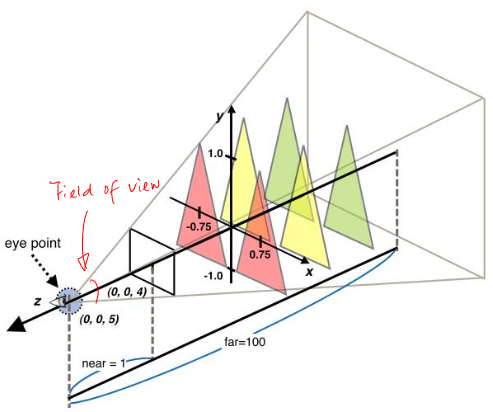
\includegraphics[scale=0.7]{setperspective}
\end{center}
Parameters:
\begin{enumerate}
	\item Field of view (in terms of angle)
	\item Aspect ratio
	\item Near plane
	\item Far plane
\end{enumerate}
\begin{minted}{javascript}
// Calculate the view matrix and the projection matrix
modelMatrix.setTranslate(0.75,0,0); // Translate 0.75 units along the positive x axis
viewMatrix.setLookAt(0,0,5,0,0,-100,0,1,0);
projMatrix.setPerspective(30, canvas.width/canvas.height,1,100);
// Pass the model, view and projection matrix to the uniform variable respectively
gl.uniformMatrix4fv(u_ModelMatrix, false, modelMatrix.elements);
gl.uniformMatrix4fv(u_ViewMatrix, false, viewMatrix.elements);
gl.uniformMatrix4fv(u_ProjMatrix, false, projMatrix.elements);
// Draw the triangles
gl.drawArrays(gl.TRIANGLES,0,n)
\end{minted}









\end{document}